% LaTeX-Vorlage Medizintechnik Projektarbeit
% Alexander Ruppel
% veraendert von Eva Eibenberger 
% veraendert von Stephan Seitz

% %%%%%%%%%%%%%%%%%%%%%%%%%%%%%%%%%%%%%%%%%%%%%%%%%%%%%%
% Please change the title of the project work, add your name 
% and matriculation number and set the language of your project 
% report 
% %%%%%%%%%%%%%%%%%%%%%%%%%%%%%%%%%%%%%%%%%%%%%%%%%%%%%%
\documentclass[%
	a4paper, %
	12pt, %
	english, % set to english if you want to write in English
	bibtotoc %
]{scrartcl}

% Gruppe: Nummer der Projektarbeit

% Thema der Projektarbeit
\newcommand{\titel}{Title}

% Studentenname und Matrikelnummer 
\newcommand{\erster}{Peter Pan}		% Student 1: Vorname Nachname
\newcommand{\mnreins}{1234567}		% Student 1: Matrikelnummer

\newcommand{\todo}[1]{{\color{blue}{TODO: {#1}}}} 
\newcommand{\sltn}[1]{{\color{red}{SOL: {#1}}}} 
\usepackage{xcolor}
\usepackage{enumitem}


% in header Spache einstellen!
\input{header}

\begin{document}

% LaTeX-Vorlage Medizintechnik Projektarbeit
% Wintersemster 2009/10
% Alexander Ruppel
% veraendert von Eva Eibenberger 
% veraendert von Paul Stöwer
% veraendert von Mischa Dombrowski

% %%%%%%%%%%%%%%%%%%%%%%%%%%%%%%%%%%%%%%%%%%%%%%%%%%%%%%
% Diese Datei muss NICHT veraendert werden
% %%%%%%%%%%%%%%%%%%%%%%%%%%%%%%%%%%%%%%%%%%%%%%%%%%%%%%

\begin{titlepage}

\begin{center}
Friedrich-Alexander-Universit\"at Erlangen-N\"urnberg\\
Artificial Intelligence in Biomedical Engineering\\
W3-Professur für Image Data Exploration and Analysis\\
Prof.\ B.\ Kainz\\
W3-Professur für Computational Imaging\\
Prof.\ F.\ Knoll\\


\vspace*{9em}

{\huge \textbf{\textsf{Medizintechnik II}}}\\[.3em]
{Projektarbeit}\\[.3em]
{Sommersemester 2023}\\

\vspace*{9em}

{\huge \textbf{\textsf{\titel}}}\\[.7em]
{\today}
\end{center}

\vfill% {
\begin{tabbing}
	\hspace*{5cm} \= Vorname Nachname \hspace*{4em} \= Matrikelnummer \kill
	Studierende*r:\> \erster \> \mnreins \\
%	\ifthenelse{\equal{\student}{\erster}}{\textbf{\erster} \> \textbf{\mnreins}}{\erster \> \mnreins} \\
%	\ifthenelse{\equal{\student}{\zweiter}}{\textbf{\zweiter} \> \textbf{\mnrzwei}}{\zweiter \> \mnrzwei} \\
%	\ifthenelse{\equal{\student}{\dritter}}{\textbf{\dritter} \> \textbf{\mnrdrei}}{\dritter \> \mnrdrei} \\
%	\ifthenelse{\equal{\student}{\vierter}}{\textbf{\vierter} \> \textbf{\mnrvier}}{\vierter \> \mnrvier} \\
%	\ifthenelse{\equal{\student}{\fuenfter}}{\textbf{\fuenfter} \> \textbf{\mnrfuenf}}{\fuenfter \> \mnrfuenf} \\
\end{tabbing}
%}

\end{titlepage}


% Inhaltsverzeichnis
\tableofcontents
\newpage

% Dateien, die den Text enthalten
\section{Introduction}%
\label{sec:einleitung}
\todo{What is MRI?}

\todo{Image acquisition}

\todo{Advantages and disadvantages}

\todo{Overview of the project}

\section{Methods}
\subsection{k-Space}

\todo{Explanation of k-space by referencing equation and figures}

\todo{Figure \ref{fig:real_imag} shows \dots} % reference all figures in text! 


\begin{equation}
    r =  \\
\end{equation}
\begin{equation} 
    \phi = \\
\end{equation}



\begin{figure}
    \centering
    \vspace{5cm}
    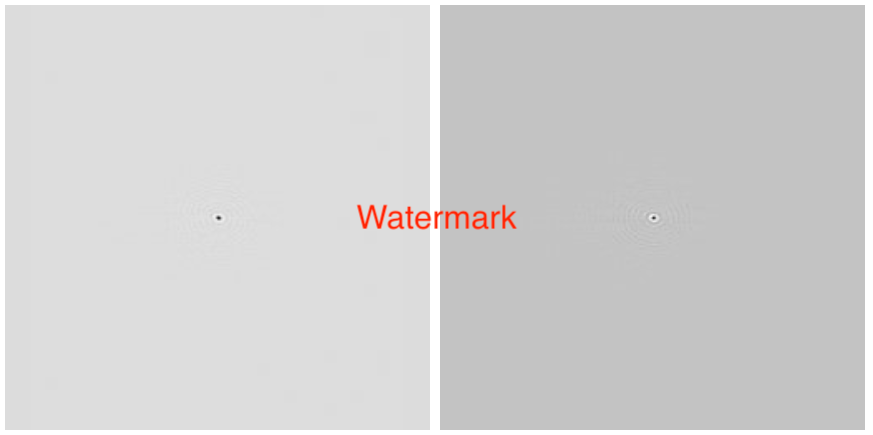
\includegraphics[width=0.6\linewidth]{latex-template-master/Grafiken/brain/realandimag.png}
    \caption{\todo{Real and imaginary part of the k-space}}
    \label{fig:real_imag}
\end{figure}

\begin{figure}
    \centering
   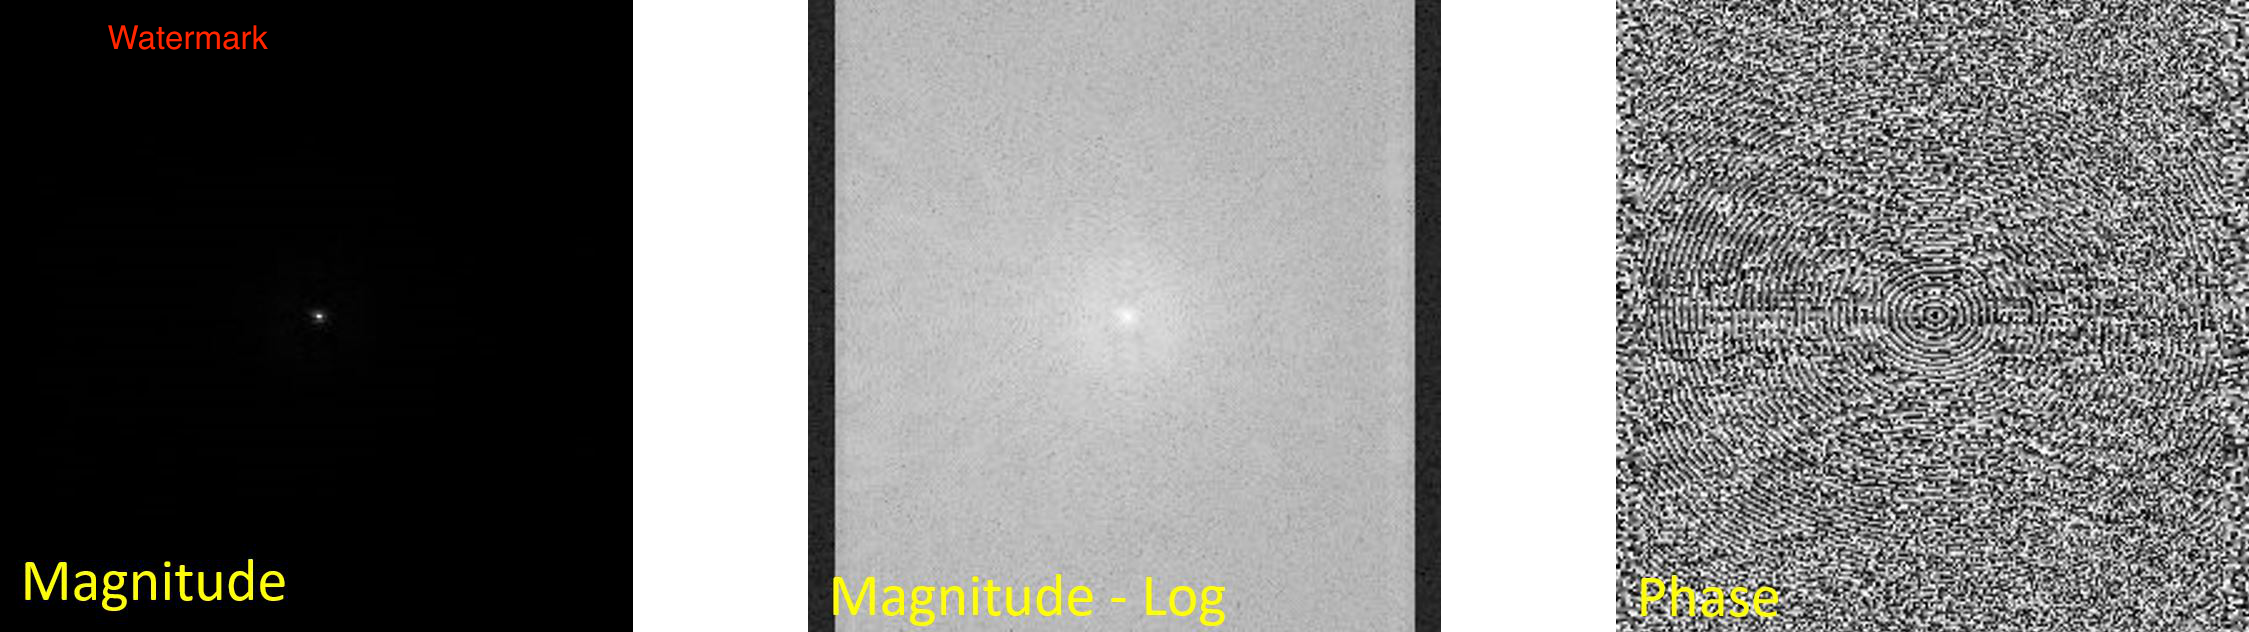
\includegraphics[width=\linewidth]{latex-template-master/Grafiken/brain/maglogphase.png}
    \caption{\todo{Magnitude, logarithmic magnitude, and phase of the k-space}}
    \label{fig:mag_phas}
\end{figure}

\newpage %CAN BE REMOVED FOR SUBMISSION


\subsection{Reconstruction}
\todo{Explain the purpose of reconstruction}

\todo{What is FFT shift}

\subsubsection{Fourier-Transformation}
\todo{Explain Fourier Transformation}


\subsubsection{MRI Image Reconstruction}
\todo{Describe and interpret reconstruction}

\todo{What happens if we revert the procedure of reconstruction? Compare Figure \ref{fig:revert}}


\begin{figure}
    \centering
    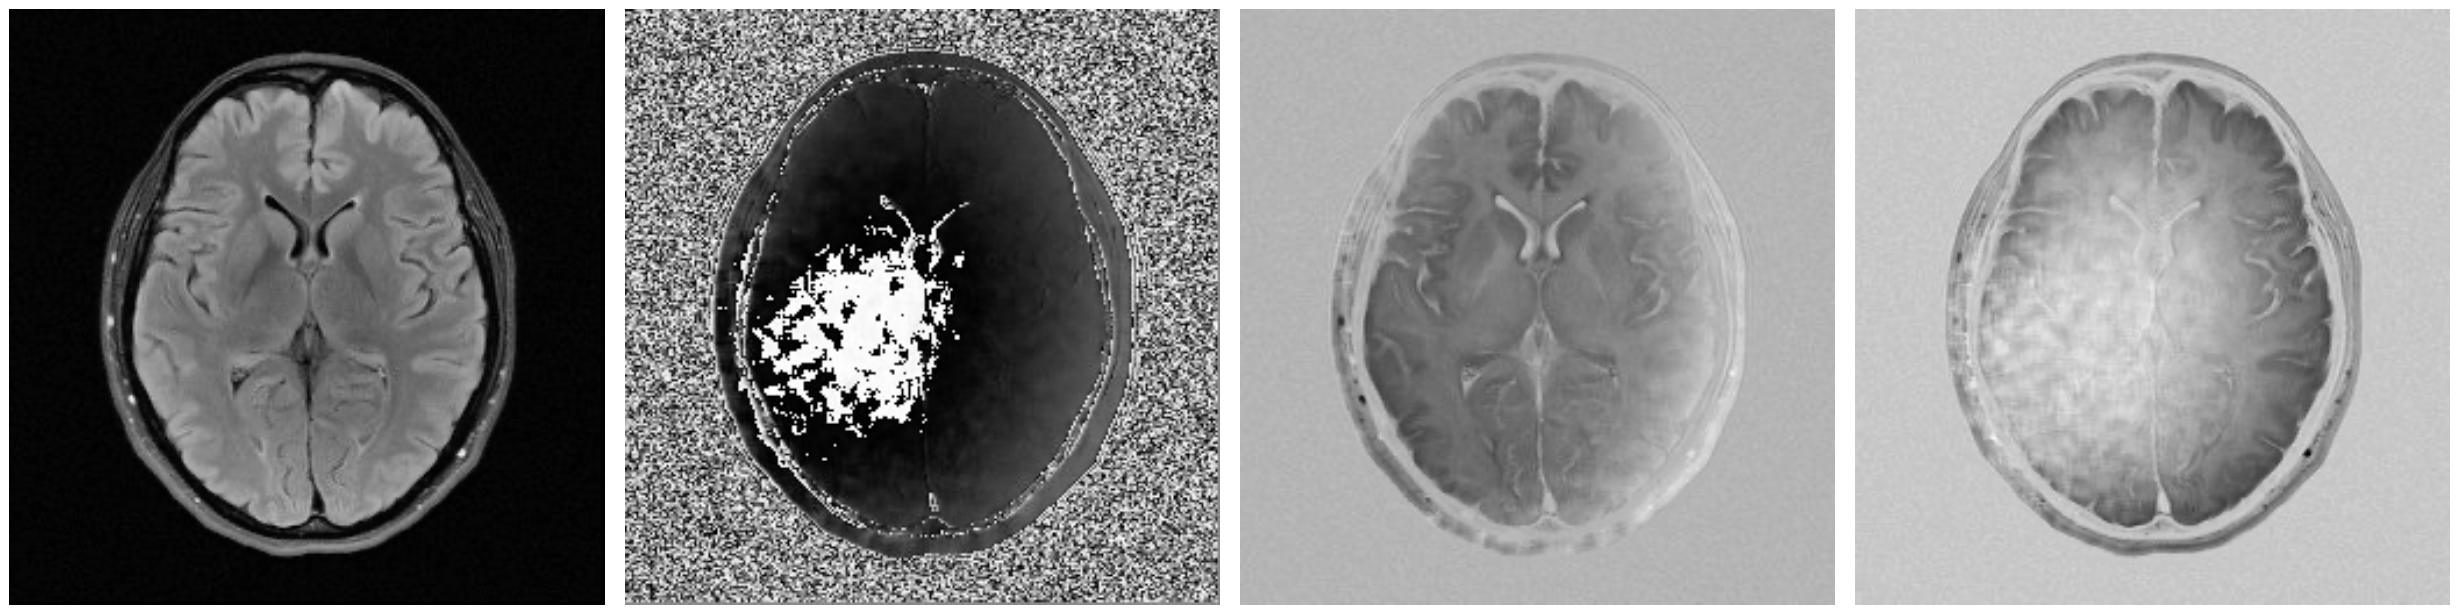
\includegraphics[width=\linewidth]{latex-template-master/Grafiken/brain/kspacereconstructed.png}
    \caption{\todo{Reconstructed image of magnitude, phase, real, and imaginary part}}
    \label{fig:reconstructed}
\end{figure}

\begin{figure}
    \centering
    \vspace{5cm} %placeholder 
    \caption{\todo{Reproduced images of the phase and the magnitude in log-scale}}
    \label{fig:revert}
\end{figure}



\subsection{Filters}
\todo{General introduction into the topic of filtering}


\subsubsection{Sinc-Filter}
\todo{Explain Sinc filtering and its effect}


\begin{figure}
    \centering
    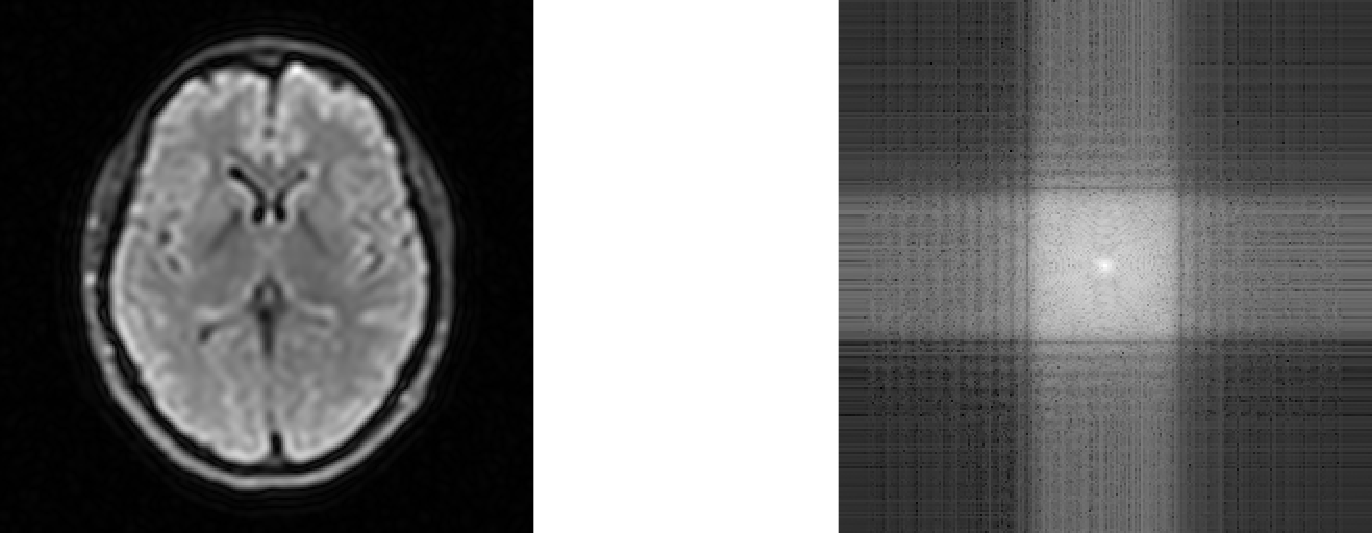
\includegraphics[width=0.9\linewidth]{latex-template-master/Grafiken/brain/sincilteredimage.png}
    \caption{\todo{The Figure shows the magnitude image and the magnitude of the k-space after application of the sinc filters.}}
    \label{fig:filterungsinc}
\end{figure}

\subsubsection{Box Multiplikation}

\todo{Explain box multiplication and compare it to the sinc filter}


\todo{Explain box multiplication with the help of Figure \ref{fig:kspacedifflevels}}



\begin{figure}
    \centering
    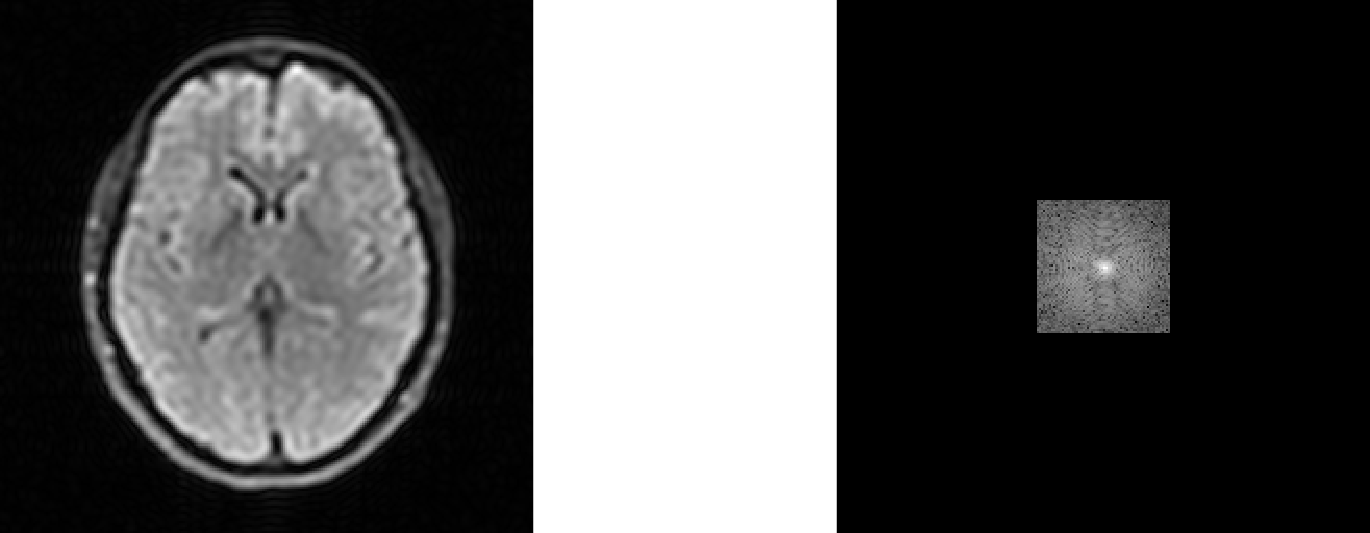
\includegraphics[width=0.9\linewidth]{latex-template-master/Grafiken/brain/boxfiltered.png}
    \caption{\todo{The Figure shows the magnitude image and the magnitude of the k-space after application of the box multiplication.}}
    \label{fig:box-mulitplikation}
\end{figure}


\begin{figure}
    \centering
    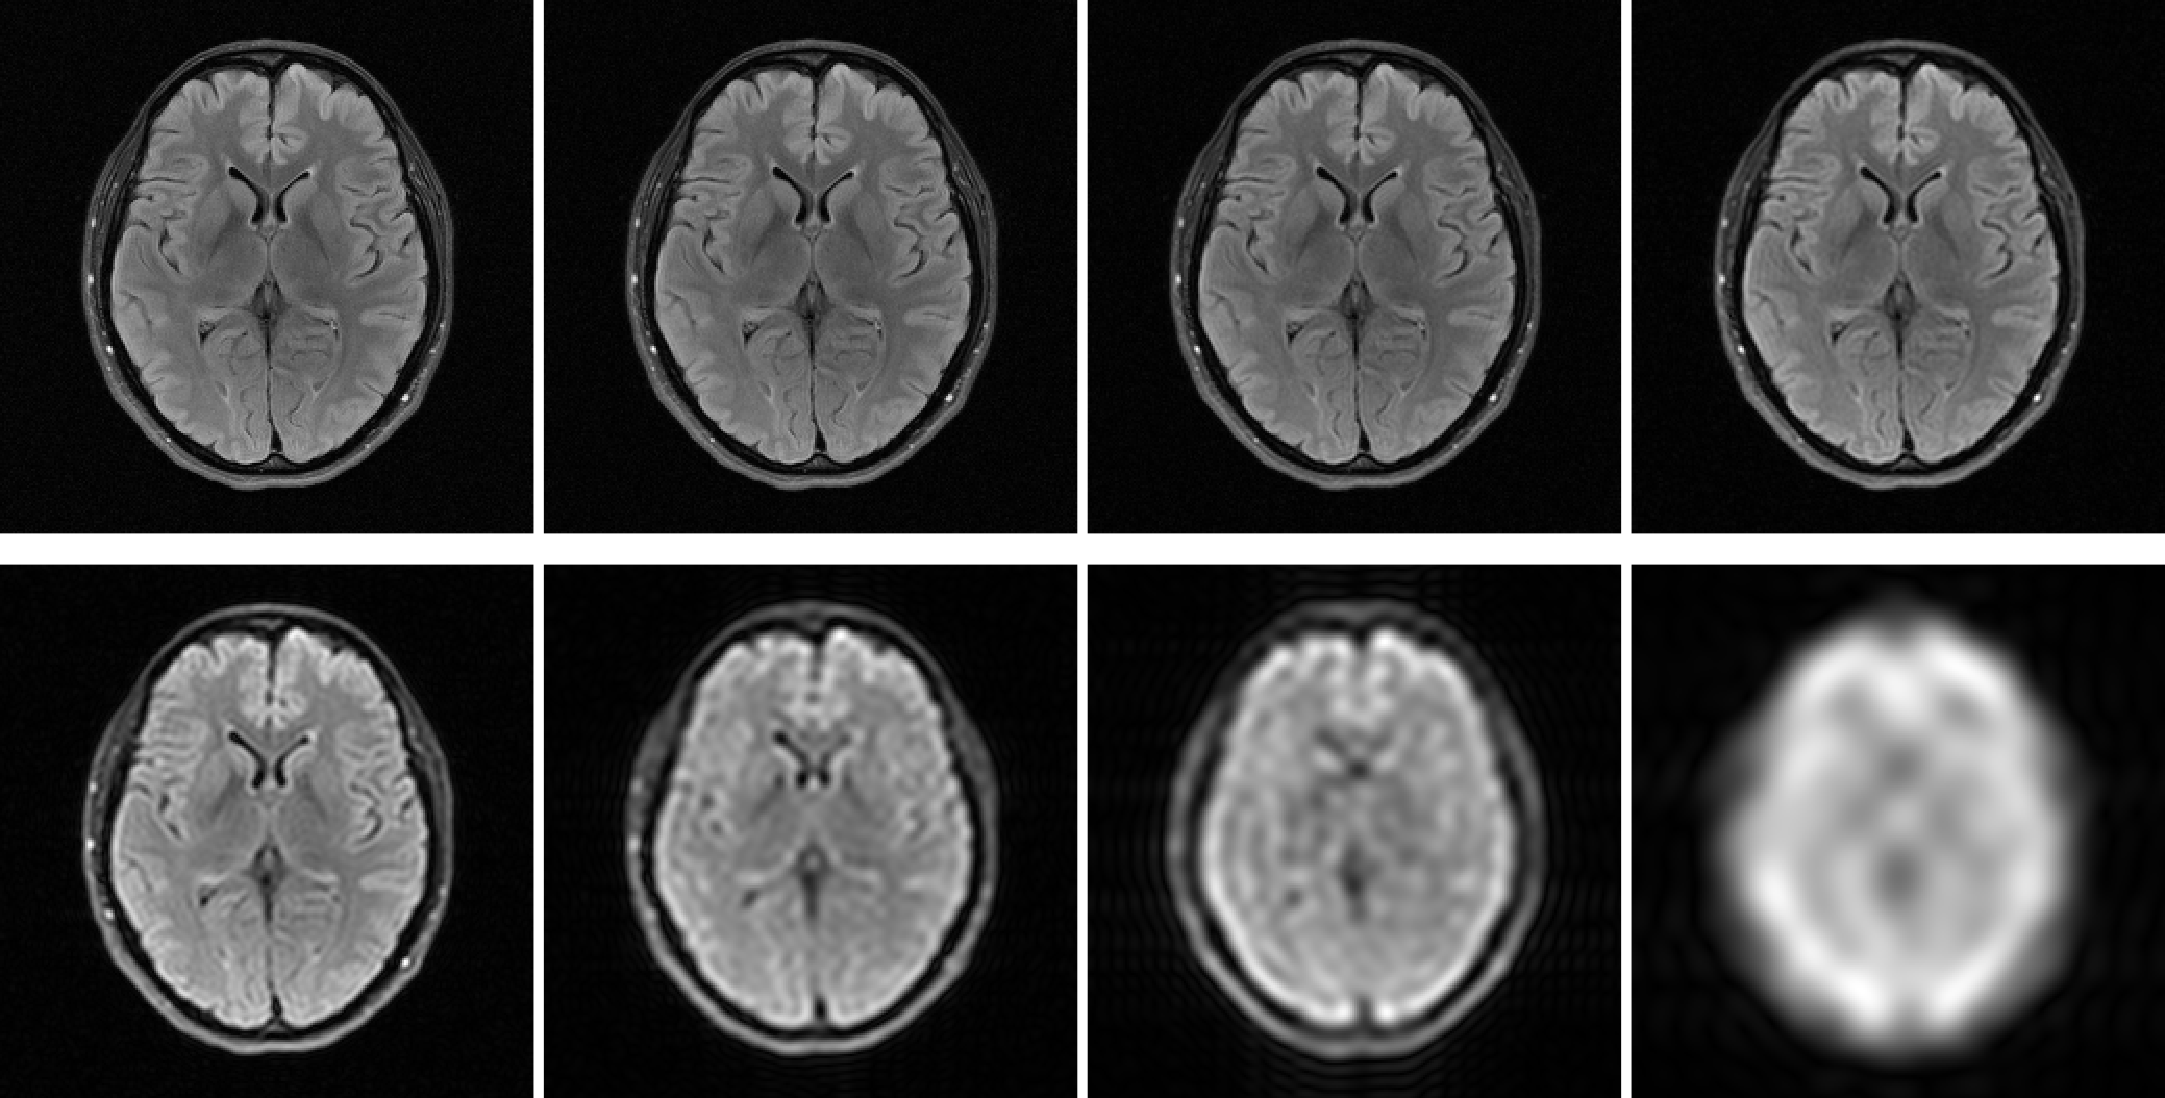
\includegraphics[width=0.9\linewidth]{latex-template-master/Grafiken/brain/kspacedifferentlevels.png}
    \caption{\todo{The Figure shows different levels of image degradation through zeroing k-space. TODO: label the different levels of zeroed k-space.}}
    \label{fig:kspacedifflevels}
\end{figure}


\newpage % TODO can be removed for final submission 

\subsection{Reducing the Image Size}

\subsubsection{Cropping k-space}

\begin{figure}
    \centering
    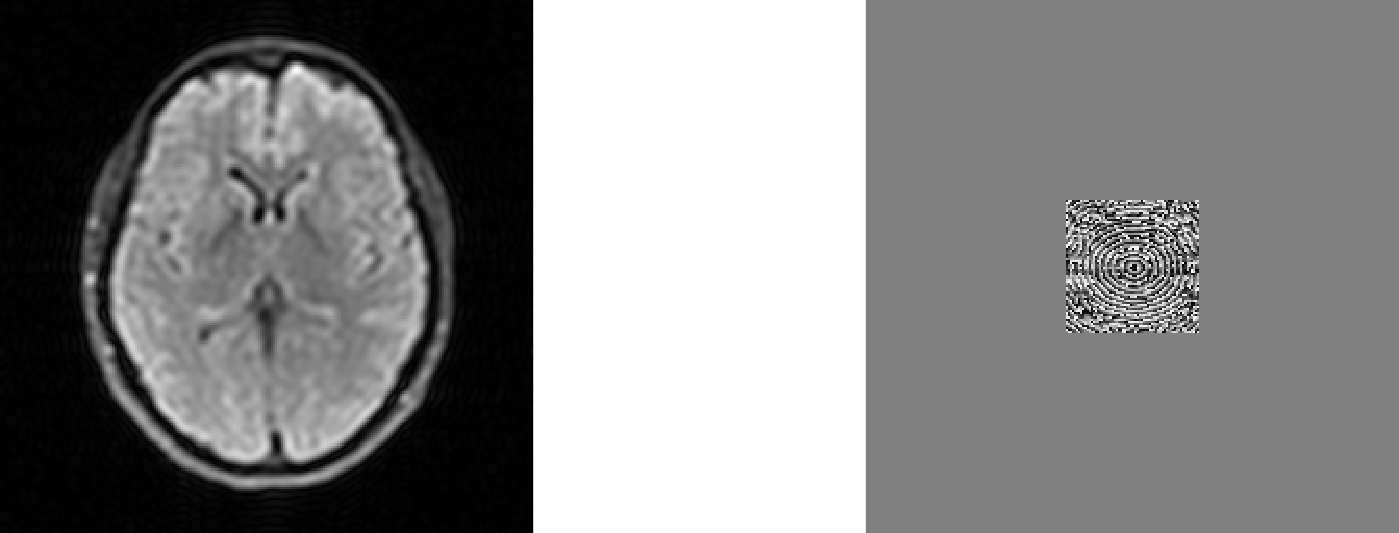
\includegraphics[width=0.9\linewidth]{latex-template-master/Grafiken/brain/croppedkspace.png}
    \caption{\todo{The Figure shows the magnitude image and the magnitude of the k-space after cropping in k-space.}}
    \label{fig:kspacecrop}
\end{figure}

\todo{Explain Cropping the k-space}



\subsubsection{Max Pooling}

\begin{figure}
    \centering
    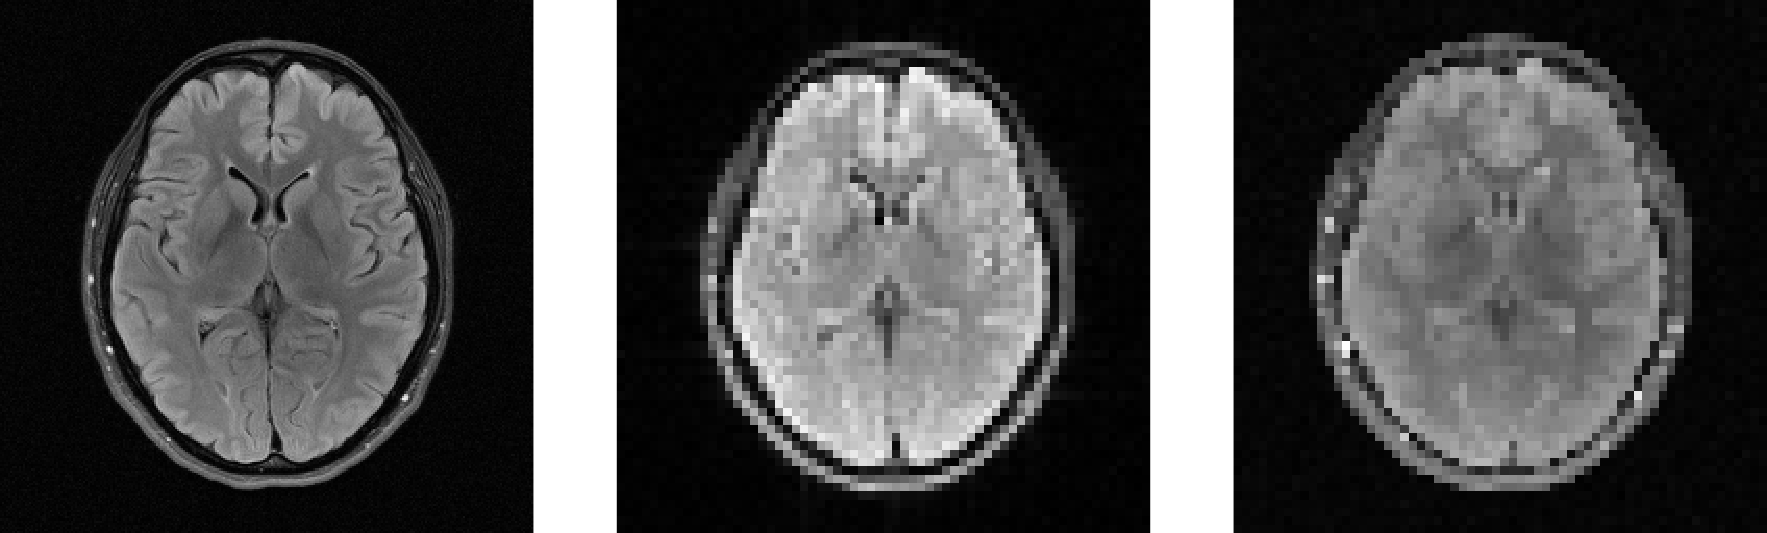
\includegraphics[width=0.9\linewidth]{latex-template-master/Grafiken/brain/maxpool.png}
    \caption{\todo{The Figure shows the original (left), the cropped k-space image (middle), and the scan after applying max pooling (right).}}
    \label{fig:maxpool}
\end{figure}

\todo{Explain Max Pooling}


\todo{Compare maxpooled and cropped k-space approach}

\section{Conclusion}

\todo{Current research \cite{Jaeger09}}



% Literaturverzeichnis
\newpage
\bibliographystyle{apalike}
\bibliography{Bib/literatur}

\end{document}
  